
\chapter{Neural Network Interfaces}
\label{app:model_interfaces}
This appendix provides an exhaustive overview of all inputs and outputs of the surrogate LSTMs provided by Frey et al.~\cite{frey_data-based_2025}. The tables are derived from the models' development documentation. Their layout has been adjusted, and the entry for $\dot m_{\mathrm{NO}_{x},\mathrm{tp}}$ [g/s], Tailpipe NOx mass-flow rate, has been standardised to match the notation used throughout this thesis.

\section{ICE - Inputs and Outputs}

\begin{table}[H]
  \centering
  \begin{tabular}{|l|l|l|}
    \hline
    \textbf{Group} & \textbf{Parameter} & \textbf{Description} \\
    \hline
    Input & $n_{ICE}$ [rpm] & Control input to all neural networks \\
    Input & $m_{fuel}$ [mg/cyl/cycle] & Fuel-mass control input \\
    Input & $T_{amb}$ [K] & Boundary input \\
    Input & $p_{amb}$ [bar] & Boundary input \\
    Output & $\tau_{ICE}$ [Nm] & Transfer output to the drivetrain model \\
    Output & $mfuel_{tot}$ [g/s] & Total burned fuel mass \\
    Output & $NO_{x_{eo}}$ [g/s] & Raw emission \\
    Output & $CO_{eo}$ [g/s] & Raw emission \\
    Output & $THC_{eo}$ [g/s] & Raw emission \\
    Output & $Tgas_{eo}$ [K] & Engine-out gas temperature \\
    Output & $\dot m_{\mathrm{NO}_{x},\mathrm{tp}}$ [g/s] & Tailpipe NOx mass-flow rate \\
    Output & $CO_{tp}$ [g/s] & Tailpipe emission \\
    Output & $CO_{2_{tp}}$ [g/s] & Tailpipe emission \\
    Output & $THC_{tp}$ [g/s] & Tailpipe emission \\
    Output & $Twall_{SCR1}$ [K] & SCR1 wall temperature \\
    Output & $Twall_{DOC}$ [K] & DOC wall temperature \\
    Output & $Tsub_{DPF}$ [K] & DPF wall temperature \\
    Output & $Twall_{SCR2}$ [K] & SCR2 wall temperature \\
    Output & $Twall_{SCR3}$ [K] & SCR3 wall temperature \\
    Output & $Tgas_{tp}$ [K] & Tailpipe gas temperature \\
    \hline
  \end{tabular}
  \caption[ICE neural-network inputs and outputs]{Inputs and outputs of the ICE neural network.}
  \label{tab:ice_io}
\end{table}

\section{Drivetrain - Inputs and Outputs}

\begin{table}[H]
  \centering
  \begin{tabular}{|l|l|l|}
    \hline
    \textbf{Group} & \textbf{Parameter} & \textbf{Description} \\
    \hline
    Input & $n_{ICE}$ [rpm] & Control input to all neural networks \\
    Input & $\tau_{ICE}$ [Nm] & Transfer input from ICE \\
    Input & $\tau_{EM2}$ [Nm] & Control input \\
    Input & \texttt{Brakemech} [\%] & Control input \\
    Output & $v_{Car}$ [km/h] & Vehicle speed \\
    Output & $SoC$ [-] & Battery state of charge \\
    \hline
  \end{tabular}
  \caption[Drivetrain neural-network inputs and outputs]{Inputs and outputs of the Drivetrain neural network.}
  \label{tab:drivetrain_io}
\end{table}

\section{Drivetrain Plus - Inputs and Outputs}

\begin{table}[H]
  \centering
  \begin{tabular}{|l|l|l|}
    \hline
    \textbf{Group} & \textbf{Parameter} & \textbf{Description} \\
    \hline
    Input & $n_{ICE}$ [rpm] & Control input to all neural networks \\
    Input & $\tau_{ICE}$ [Nm] & Transfer input from ICE \\
    Input & $\tau_{EM2}$ [Nm] & Control input \\
    Input & \texttt{Brakemech} [\%] & Control input \\
    Output & $\tau_{EM1,out}$ [Nm] & Actual EM1 torque \\
    Output & $\tau_{EM2,out}$ [Nm] & Actual EM2 torque \\
    Output & $n_{Sun}$ [rpm] & Actual sun speed \\
    Output & $n_{Ring}$ [rpm] & Actual ring speed \\
    \hline
  \end{tabular}
  \caption[Drivetrain Plus neural-network inputs and outputs]{Inputs and outputs of the Drivetrain Plus neural network.}
  \label{tab:drivetrain_plus_io}
\end{table}

\chapter{Phase~1 - Hyperparameter Optimisation Details}
\label{app:phase1_hyperparams}
This appendix chapter lists the Phase~1 hyperparameter-optimisation search space, the Optuna trial histories, and the final best hyperparameter configuration for each algorithm. The corresponding Phase~2 reward-weight optimisation diagnostics are collected separately in \autoref{app:phase2_reward_weight_optimisation}.

\section{Phase 1 - Optuna Search Spaces}
\label{app:phase1_search_spaces}

\begin{table}[H]
  \centering
  % \small
  % \setlength{\tabcolsep}{3pt}
  % \renewcommand{\arraystretch}{0.9}
  \begin{tabular}{|l|l|}
    \hline
    \textbf{Hyperparameter} & \textbf{Range / choices} \\
    \hline
    \multicolumn{2}{|l|}{\textit{Shared across all algorithms}} \\
    \texttt{net\_arch} & $\{[64,64],\,[128,128],\,[256,256],\,[128,128,128]\}$ \\
    \hline
    \multicolumn{2}{|l|}{\textit{PPO}} \\
    \texttt{learning\_rate} & log-uniform $[10^{-5},\,10^{-3}]$ \\
    \texttt{n\_steps}       & $\{1024,\,2048,\,4096\}$ \\
    \texttt{batch\_size}    & $\{64,\,128,\,256,\,512\}$ \\
    \texttt{n\_epochs}      & int $[3,\,15]$ \\
    \texttt{gamma}          & uniform $[0.95,\,0.999]$ \\
    \texttt{gae\_lambda}    & uniform $[0.9,\,1.0]$ \\
    \texttt{clip\_range}    & uniform $[0.1,\,0.3]$ \\
    \hline
    \multicolumn{2}{|l|}{\textit{SAC}} \\
    \texttt{learning\_rate}     & log-uniform $[10^{-5},\,10^{-3}]$ \\
    \texttt{batch\_size}        & $\{128,\,256,\,512,\,1024\}$ \\
    \texttt{tau}                & uniform $[10^{-3},\,2\times10^{-2}]$ \\
    \texttt{gamma}              & uniform $[0.95,\,0.999]$ \\
    \texttt{train\_freq}        & $\{1,\,4,\,8\}$ \\
    \texttt{gradient\_steps}    & $\{1,\,4,\,8\}$ \\
    \texttt{learning\_starts}   & $\{1000,\,5000,\,10000,\,20000\}$ \\
    \texttt{ent\_coef}          & $\{\text{\texttt{auto}},\,0.01,\,0.05,\,0.1,\,0.2\}$ \\
    \texttt{use\_sde}           & $\{\text{True},\,\text{False}\}$ \\
    \hline
    \multicolumn{2}{|l|}{\textit{TD3}} \\
    \texttt{learning\_rate}        & log-uniform $[10^{-5},\,10^{-3}]$ \\
    \texttt{batch\_size}           & $\{128,\,256,\,512,\,1024\}$ \\
    \texttt{tau}                   & uniform $[10^{-3},\,2\times10^{-2}]$ \\
    \texttt{gamma}                 & uniform $[0.95,\,0.999]$ \\
    \texttt{train\_freq}           & $\{1,\,4,\,8\}$ \\
    \texttt{gradient\_steps}       & $\{1,\,4,\,8\}$ \\
    \texttt{learning\_starts}      & $\{1000,\,5000,\,10000,\,20000\}$ \\
    \texttt{policy\_delay}         & $\{1,\,2,\,4\}$ \\
    \texttt{target\_policy\_noise} & uniform $[0.1,\,0.4]$ \\
    \texttt{target\_noise\_clip}   & uniform $[0.3,\,0.7]$ \\
    \texttt{action\_noise\_sigma}  & uniform $[0.05,\,0.3]$ \\
    \hline
  \end{tabular}
  \caption[Phase-1 Optuna search spaces]{Phase-1 Optuna search spaces per algorithm. The shared \texttt{net\_arch} discrete set is sampled once per trial and applied to both actor and critic networks.}
  \label{tab:hpo_search_spaces}
\end{table}

\section{Phase 1 - Optuna Trial Histories}
\label{app:phase1_trial_histories}

The following plots document the Phase~1 Optuna studies used to select the hyperparameter configurations reported in \autoref{tab:phase1_best_hyperparameters}. They are included here as optimisation diagnostics; the main results chapter focuses on the seed-wise retraining and evaluation behaviour of the selected configurations.

\begin{figure}[H]
  \centering
  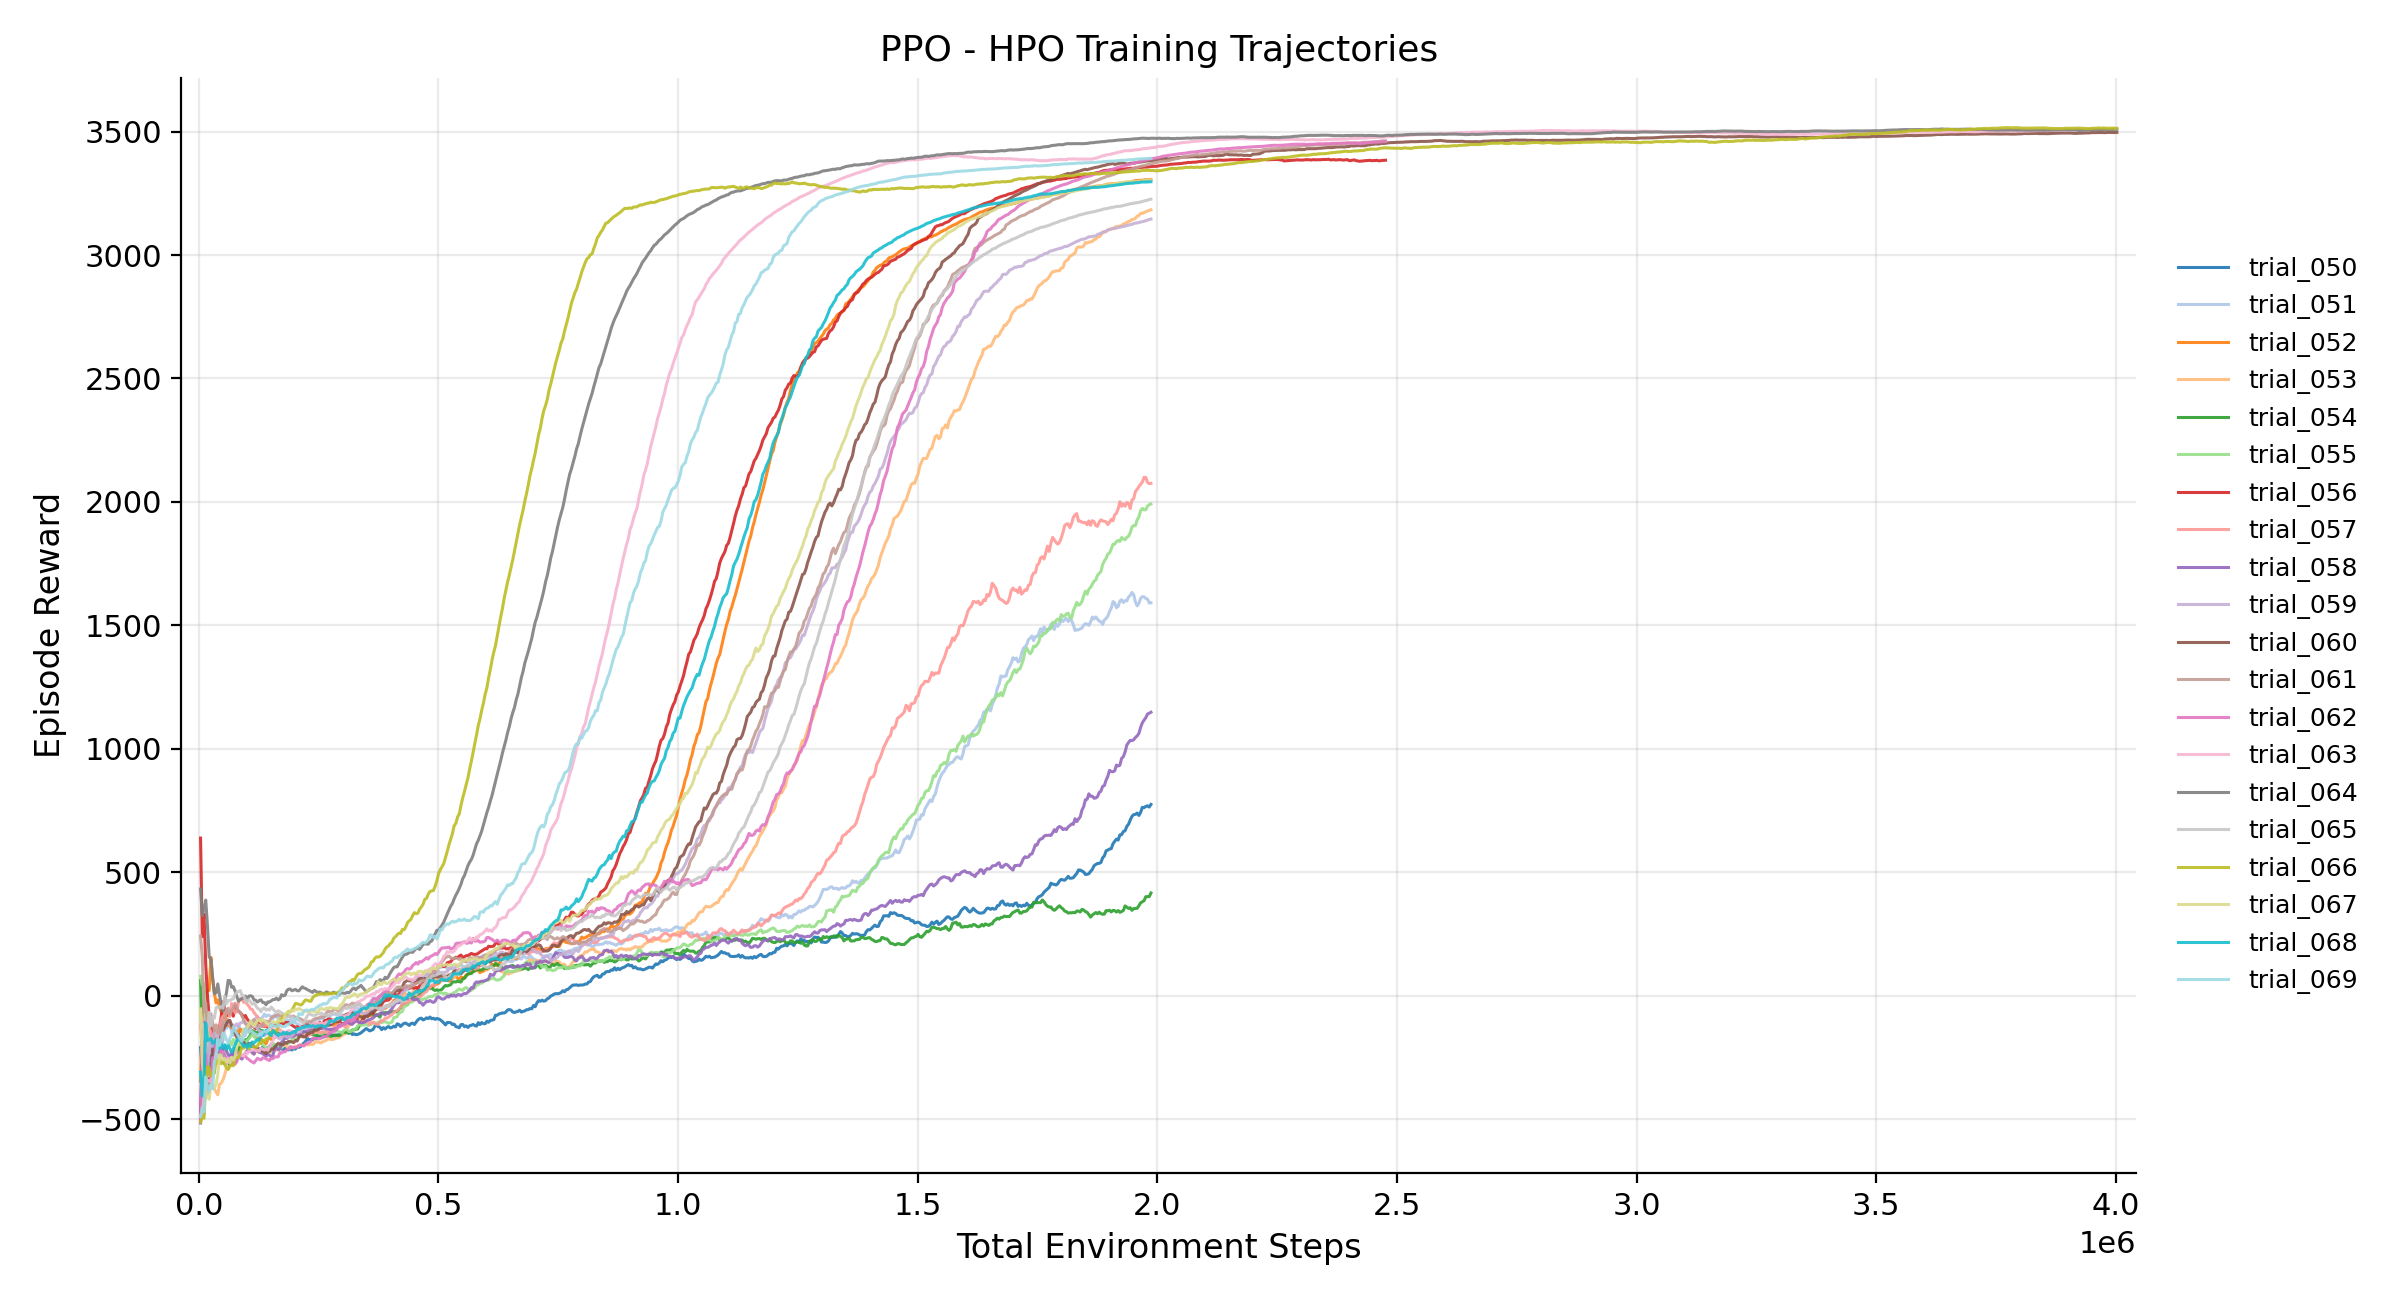
\includegraphics[width=0.85\textwidth]{imgs/plots/phase1/ppo/ppo_trials.png}
  \caption[PPO Optuna trials in Phase~1]{Optuna trial results for PPO in Phase~1; curves are smoothed via moving average over 80 episodes.}
  \label{fig:phase1_ppo_trials}
\end{figure}

\begin{figure}[H]
  \centering
  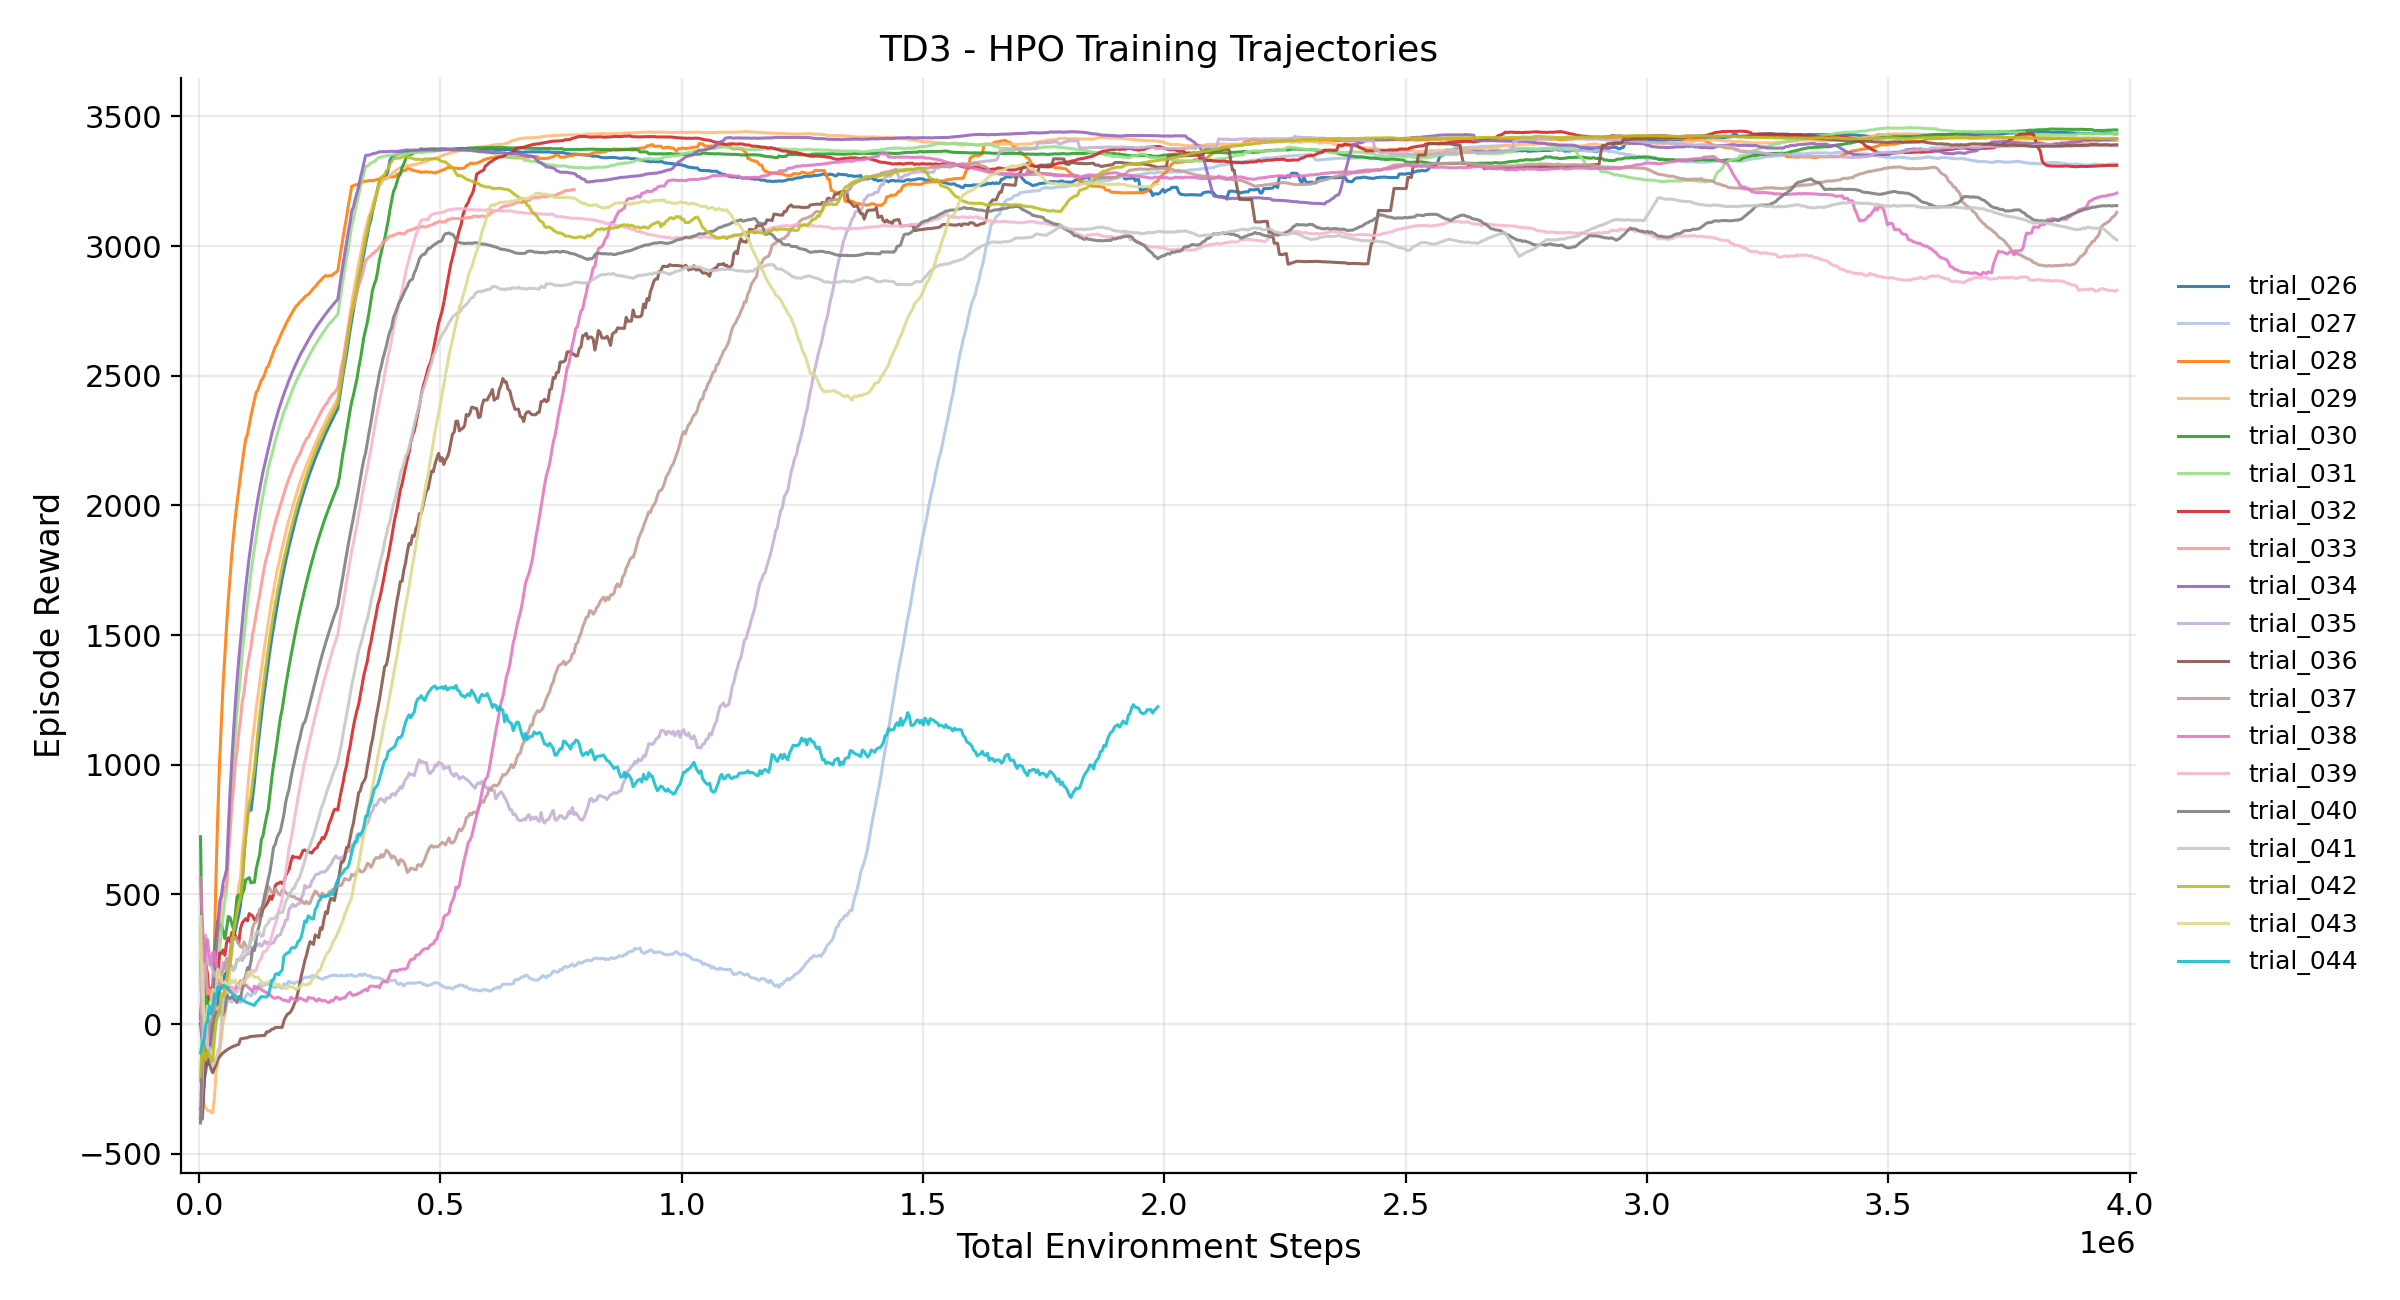
\includegraphics[width=0.85\textwidth]{imgs/plots/phase1/td3/td3_trials.png}
  \caption[TD3 Optuna trials in Phase~1]{Optuna trial results for TD3 in Phase~1; curves are smoothed via moving average over 80 episodes.}
  \label{fig:phase1_td3_trials}
\end{figure}

\begin{figure}[H]
  \centering
  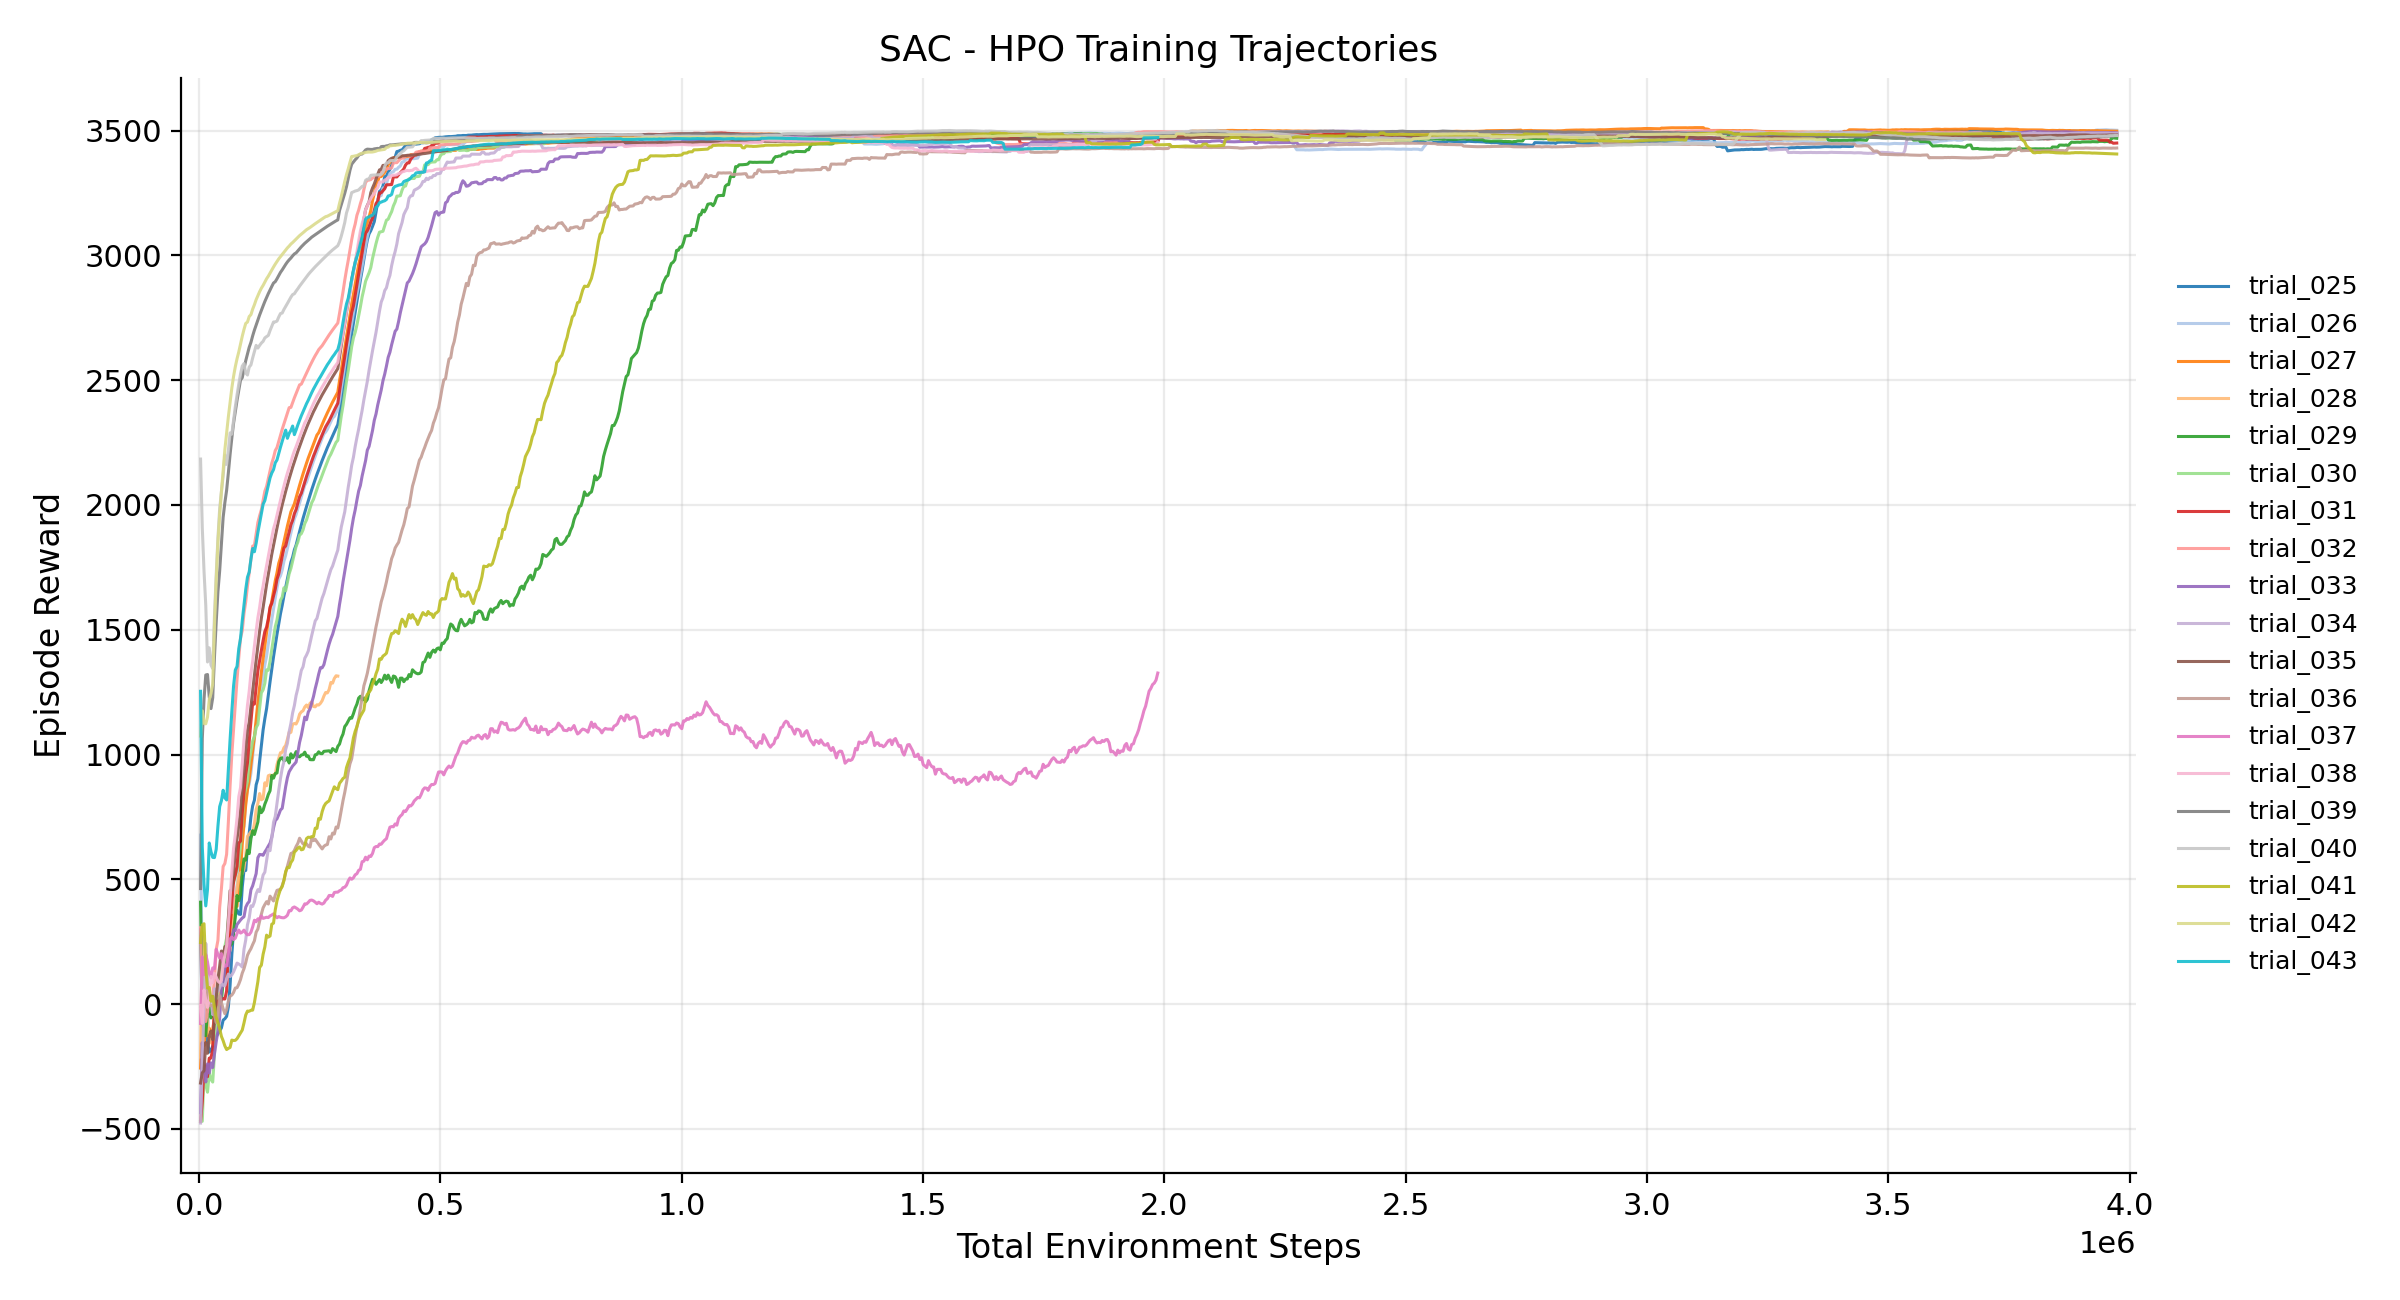
\includegraphics[width=0.85\textwidth]{imgs/plots/phase1/sac/sac_trials.png}
  \caption[SAC Optuna trials in Phase~1]{Optuna trial results for SAC in Phase~1; curves are smoothed via moving average over 80 episodes.}
  \label{fig:phase1_sac_trials}
\end{figure}


\section{Phase 1 - Best Hyperparameter Sets}
\label{app:phase1_best_sets}

\begin{table}[H]
  \centering
  \begin{tabular}{|l|c|c|c|}
    \hline
    \textbf{Parameter} & \textbf{PPO} & \textbf{SAC} & \textbf{TD3} \\
    \hline
    \texttt{learning\_rate} & $1.28 \times 10^{-5}$ & $9.20 \times 10^{-4}$ & $1.79 \times 10^{-4}$ \\
    \texttt{gamma} & 0.9647 & 0.9601 & 0.9647 \\
    \texttt{batch\_size} & 64 & 512 & 1024 \\
    \texttt{net\_arch} & [256, 256] & [128, 128, 128] & [128, 128] \\
    \texttt{n\_steps} & 2048 & -- & -- \\
    \texttt{train\_freq} & -- & 1 & 1 \\
    \texttt{gradient\_steps} & -- & 8 & 8 \\
    \texttt{n\_epochs} & 11 & -- & -- \\
    \texttt{gae\_lambda} & 0.965 & -- & -- \\
    \texttt{clip\_range} & 0.203 & -- & -- \\
    \texttt{tau} & -- & 0.0080 & 0.0082 \\
    \texttt{learning\_starts} & -- & 1{,}000 & 20{,}000 \\
    \texttt{ent\_coef} & -- & \texttt{auto} & -- \\
    \texttt{use\_sde} & -- & False & -- \\
    \texttt{policy\_delay} & -- & -- & 1 \\
    \texttt{target\_policy\_noise} & -- & -- & 0.116 \\
    \texttt{target\_noise\_clip} & -- & -- & 0.699 \\
    \texttt{action\_noise\_sigma} & -- & -- & 0.144 \\
    \hline
  \end{tabular}
  \caption[Best Phase-1 hyperparameter configurations]{Best hyperparameter configurations identified for Phase~1 across all evaluated \ac{RL} algorithms.}
  \label{tab:phase1_best_hyperparameters}
\end{table}

\chapter{Phase~2 - Reward Weight Optimisation Details}
\label{app:phase2_reward_weight_optimisation}

This appendix chapter documents the Phase~2 reward-weight Optuna studies used to select the emission and quadratic \ac{SOC} weights reported in \autoref{tab:phase2_best_trials}. The plots are included as additional diagnostics; the main results chapter reports the selected Phase~2 reward weights and trial results in \autoref{tab:reward_weights} and \autoref{tab:phase2_best_trials}, respectively.

\section{Phase 2 - Reward-Weight Trial Histories}
\label{app:phase2_reward_trial_histories}

\begin{figure}[H]
  \centering
  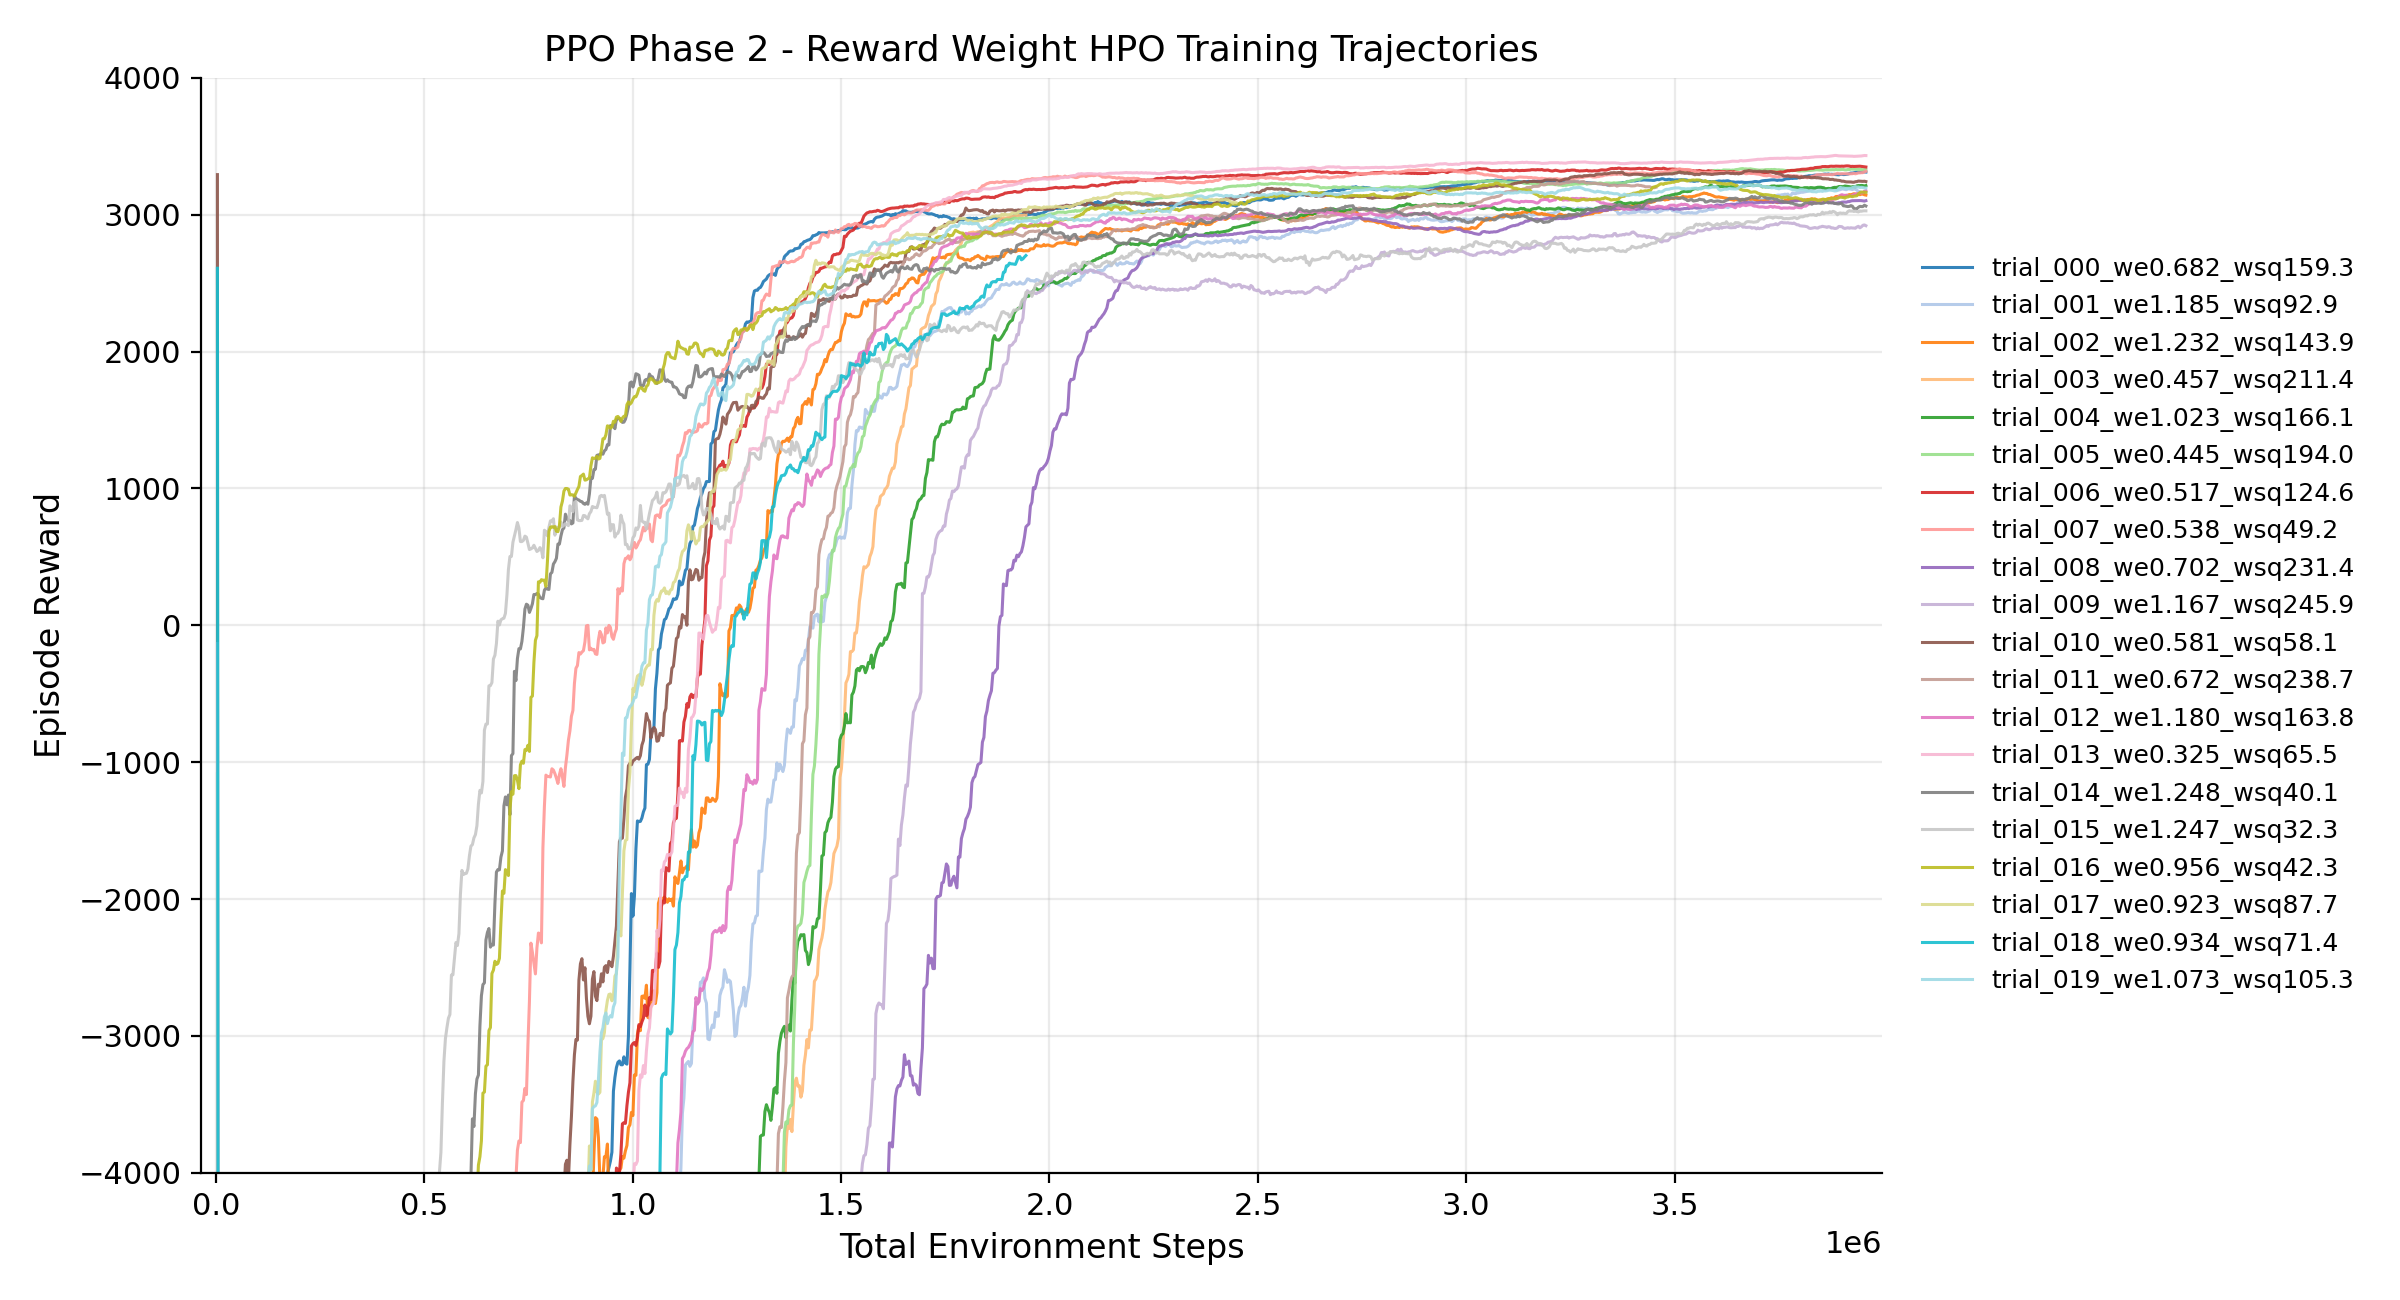
\includegraphics[width=0.85\textwidth]{imgs/plots/phase2/ppo/ppo_reward_trials.png}
  \caption[PPO reward-weight Optuna trials in Phase~2]{Reward-weight Optuna trial results for PPO in Phase~2. The trials tune the active emission and quadratic \ac{SOC} weights while keeping the Phase~1 speed-tracking configuration fixed; curves are smoothed via moving average over 80 episodes.}
  \label{fig:phase2_ppo_reward_trials}
\end{figure}

\begin{figure}[H]
  \centering
  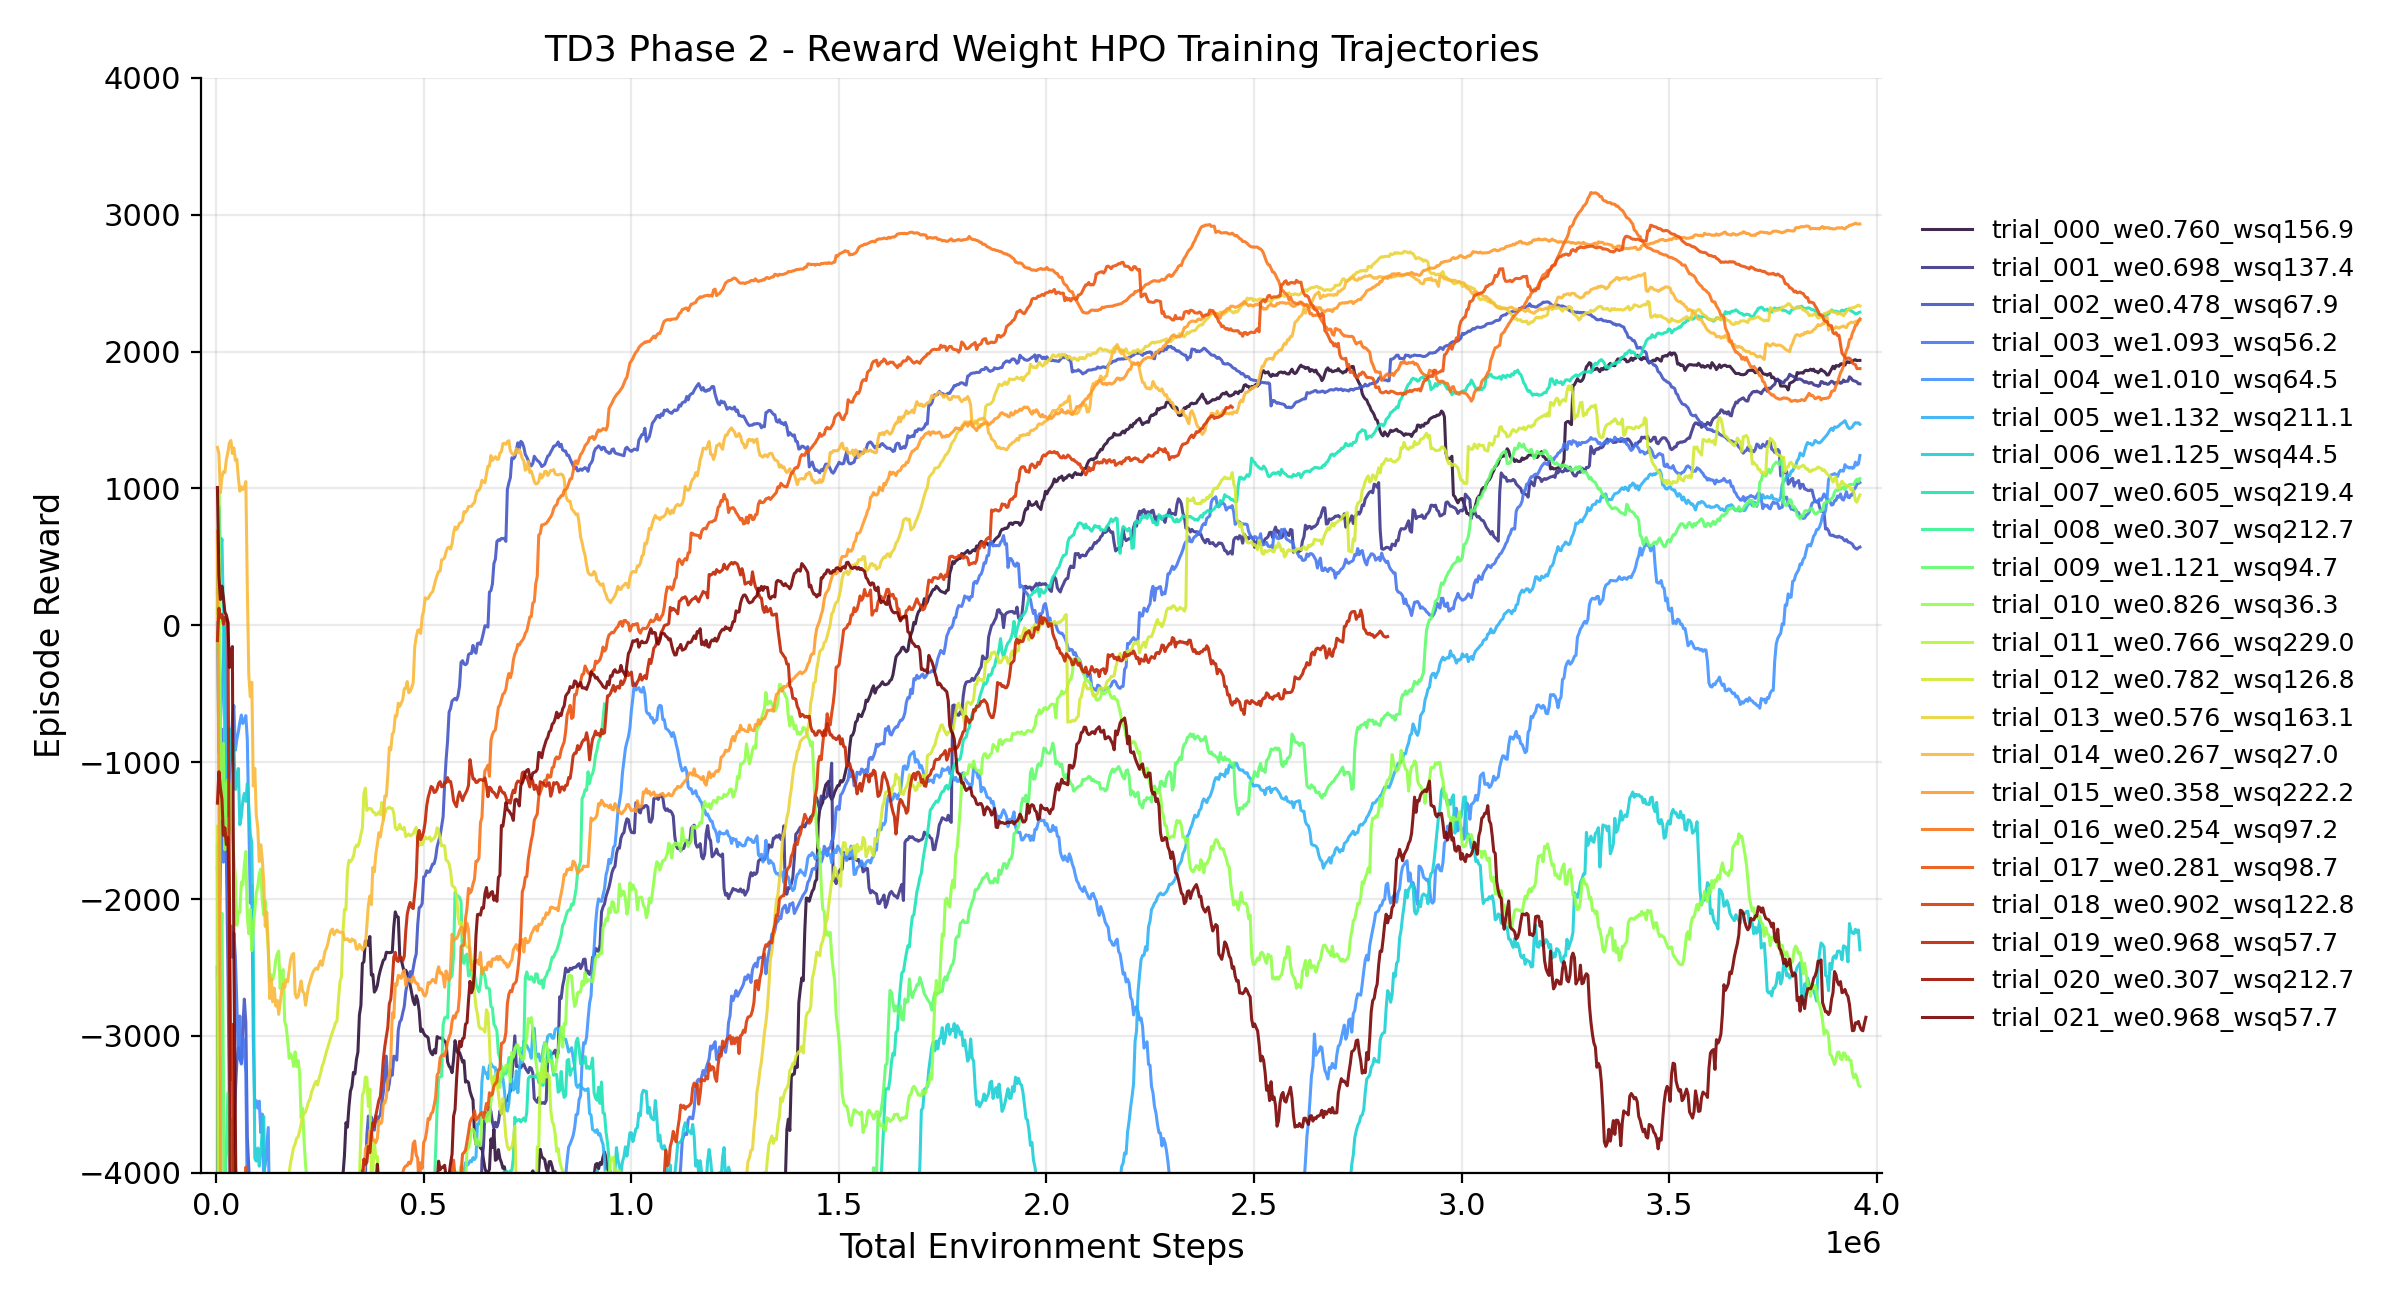
\includegraphics[width=0.85\textwidth]{imgs/plots/phase2/td3/td3_reward_trials.png}
  \caption[TD3 reward-weight Optuna trials in Phase~2]{Reward-weight Optuna trial results for TD3 in Phase~2. The trials tune the active emission and quadratic \ac{SOC} weights while keeping the Phase~1 speed-tracking configuration fixed; curves are smoothed via moving average over 80 episodes.}
  \label{fig:phase2_td3_reward_trials}
\end{figure}

\begin{figure}[H]
  \centering
  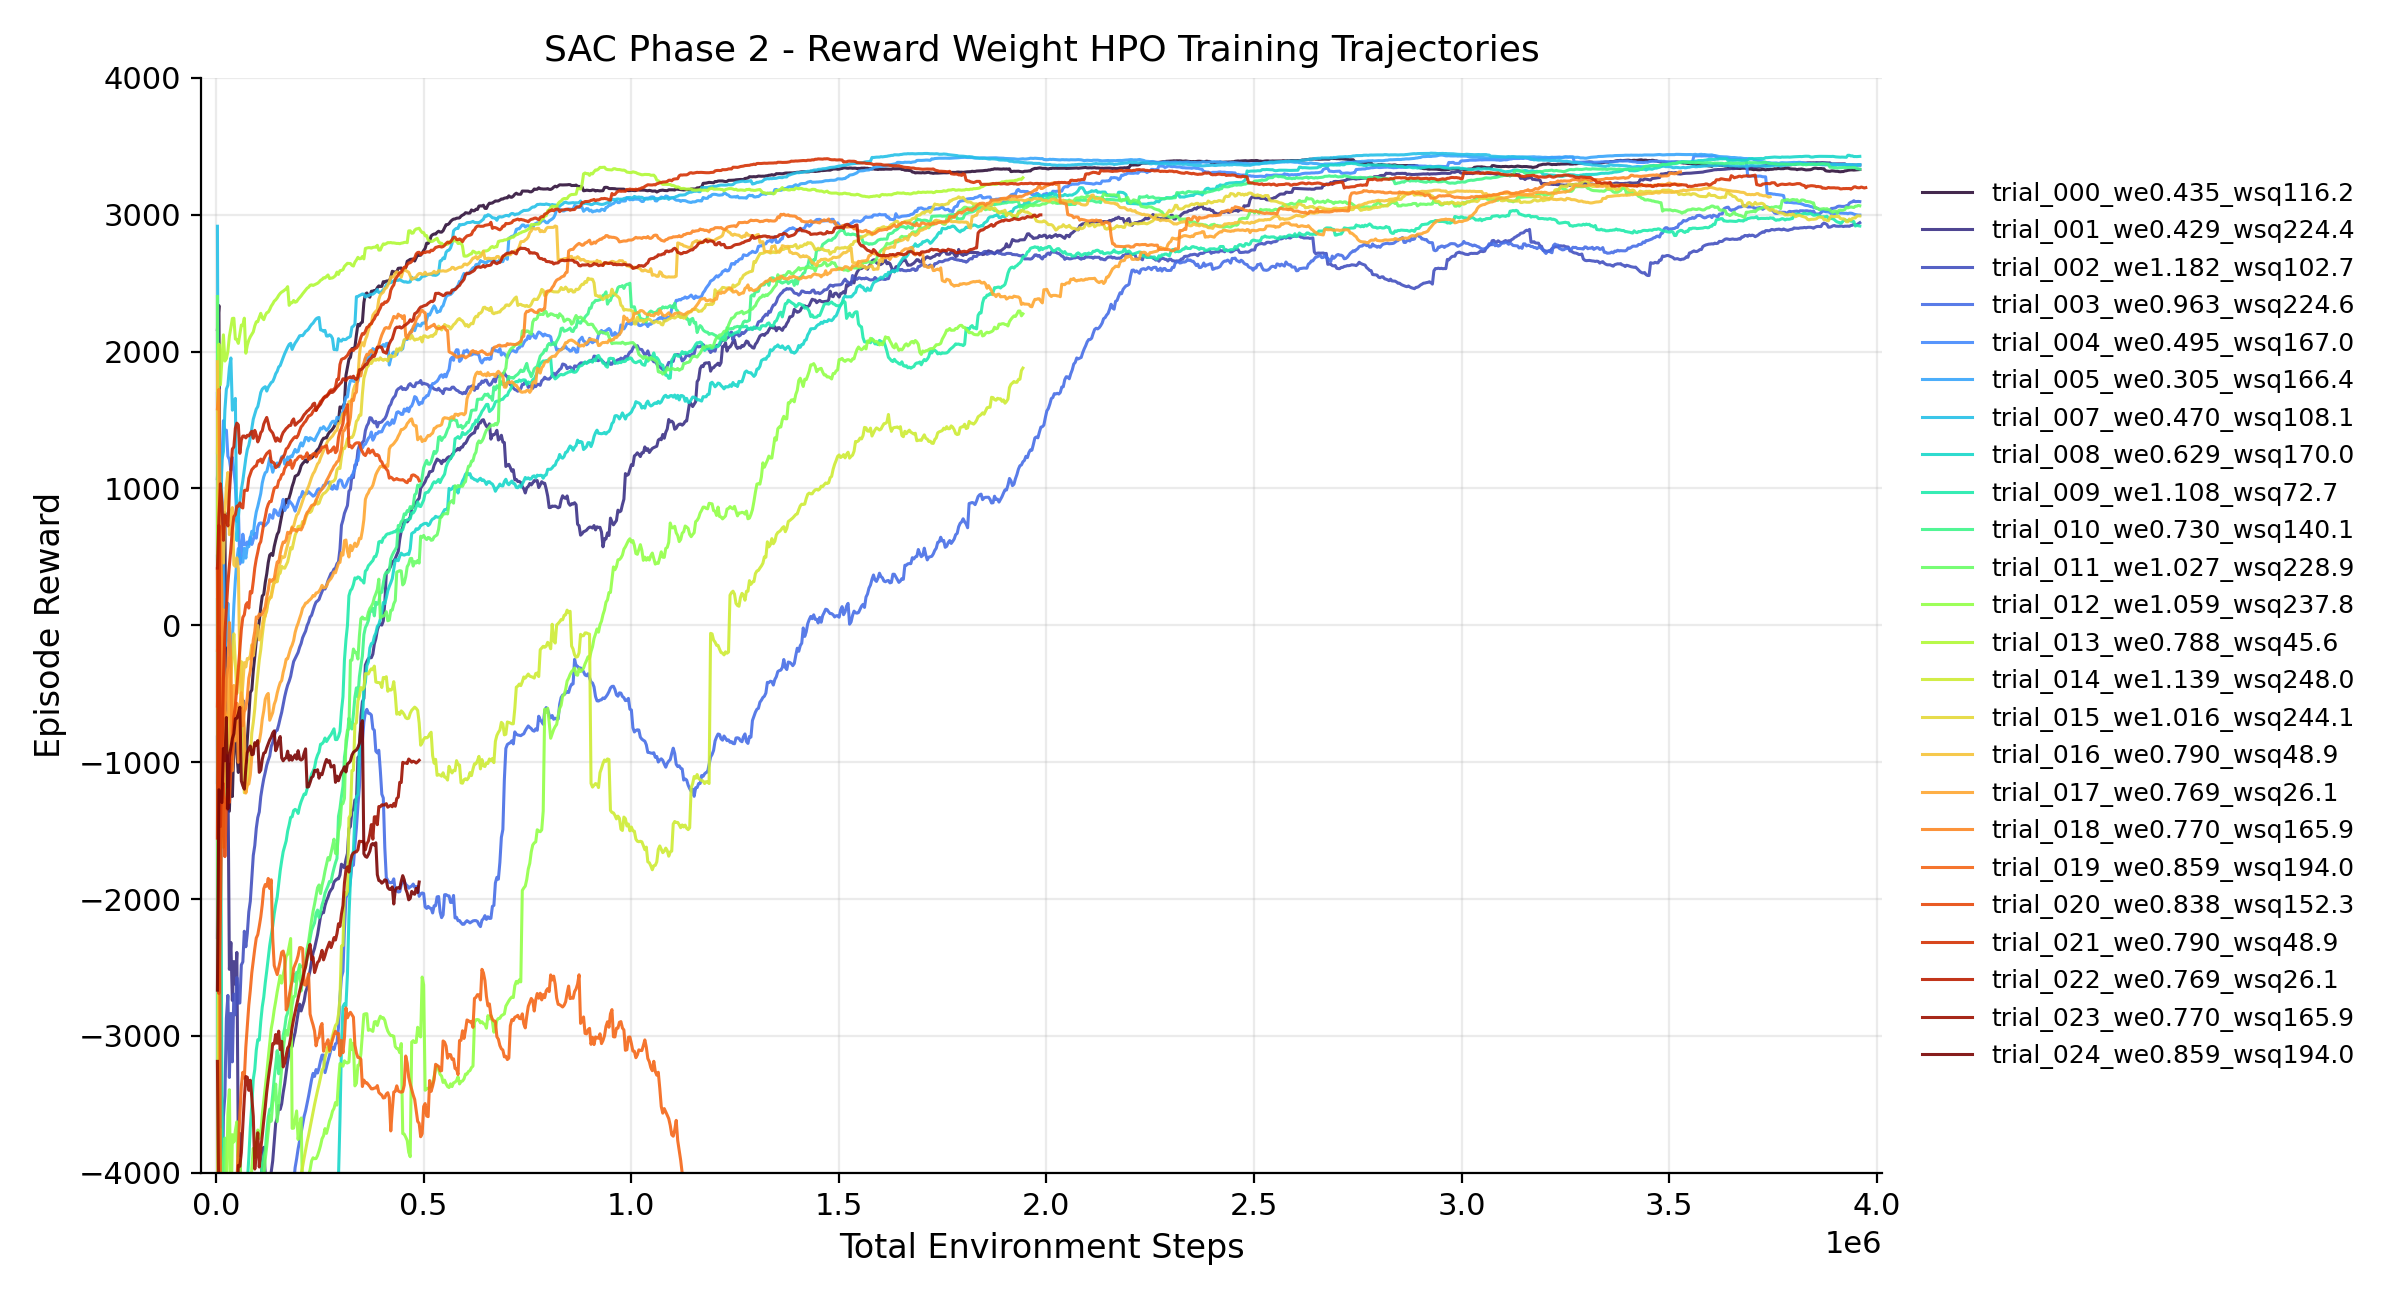
\includegraphics[width=0.85\textwidth]{imgs/plots/phase2/sac/sac_reward_trials.png}
  \caption[SAC reward-weight Optuna trials in Phase~2]{Reward-weight Optuna trial results for SAC in Phase~2. The trials tune the active emission and quadratic \ac{SOC} weights while keeping the Phase~1 speed-tracking configuration fixed; curves are smoothed via moving average over 80 episodes.}
  \label{fig:phase2_sac_reward_trials}
\end{figure}
